\section{HAT}
Pro ovládání výše popsaného hardwaru je zapotřebí několik specifických obvodů.
Kvůli jejich specifičnosti tyto obvody nejsou volně dostupné k zakoupení na předem vytvořených destičkách. Proto bylo zapotřebí je z jednotlivých součástek vyrobit na míru.

Obvody byly navrženy v programu KiCad...\fxnote{bud spojit vety, nebo k prvni neco jeste dopsat}
Následně pro ně v tomtéž programu byla nadesignována deska plošných spojů. Na této desce se vyskytují obvody \fxnote{todo dac+amps, bat\_probe, -15V}.
Kromě nich byly na desku přidány konektory k jednotlivým barevným vstupům laseru, LCD displeji a k rotačnímu enkodéru, které jsou přímo napojeny na 40 pinový GPIO konektor Raspberry Pi.
Deska byla designována jako tzv. HAT, to znamená, že sama na tomto konektoru drží a nezabírá o moc víc místa, než samotné Raspberry Pi.
\fxnote{TODO: obrazek desky (maybe mounted)}


\subsection{obvod pro generování analogového signálu}
Jak popsáno v sekci \ref{sec:my-galvos}, řídící deska galvanometrů přijmá dva bipolární diferenciální analogové signály v rozpětí $-5$~V až $+5$~V.

Obvod, který se stará o vytváření tohoto signálu je založený na obvodu ze zdroje \cite{lasershow-with-real-galvos}.
Vytváření tohoto signálu je rozděleno do dvou částí. Nejdříve DAC (digital-to-analog converter, D/A převodník) připojený k RPi vytvoří signál v rozpětí 0 až 5~V a následně je tento signál pomocí operačního zesilovače převeden na požadované rozpětí, tj. $-15$~V až $+15$~V.
Jednotlivé části tohoto obvodu jsou blíže popsány v následujících kapitolách. Celé zapojení je vidět na obrázku \ref{fig:dac_board}.
\fxnote{unreadable text, make schem more compact}
\begin{figure}[!htb]
  \centering
  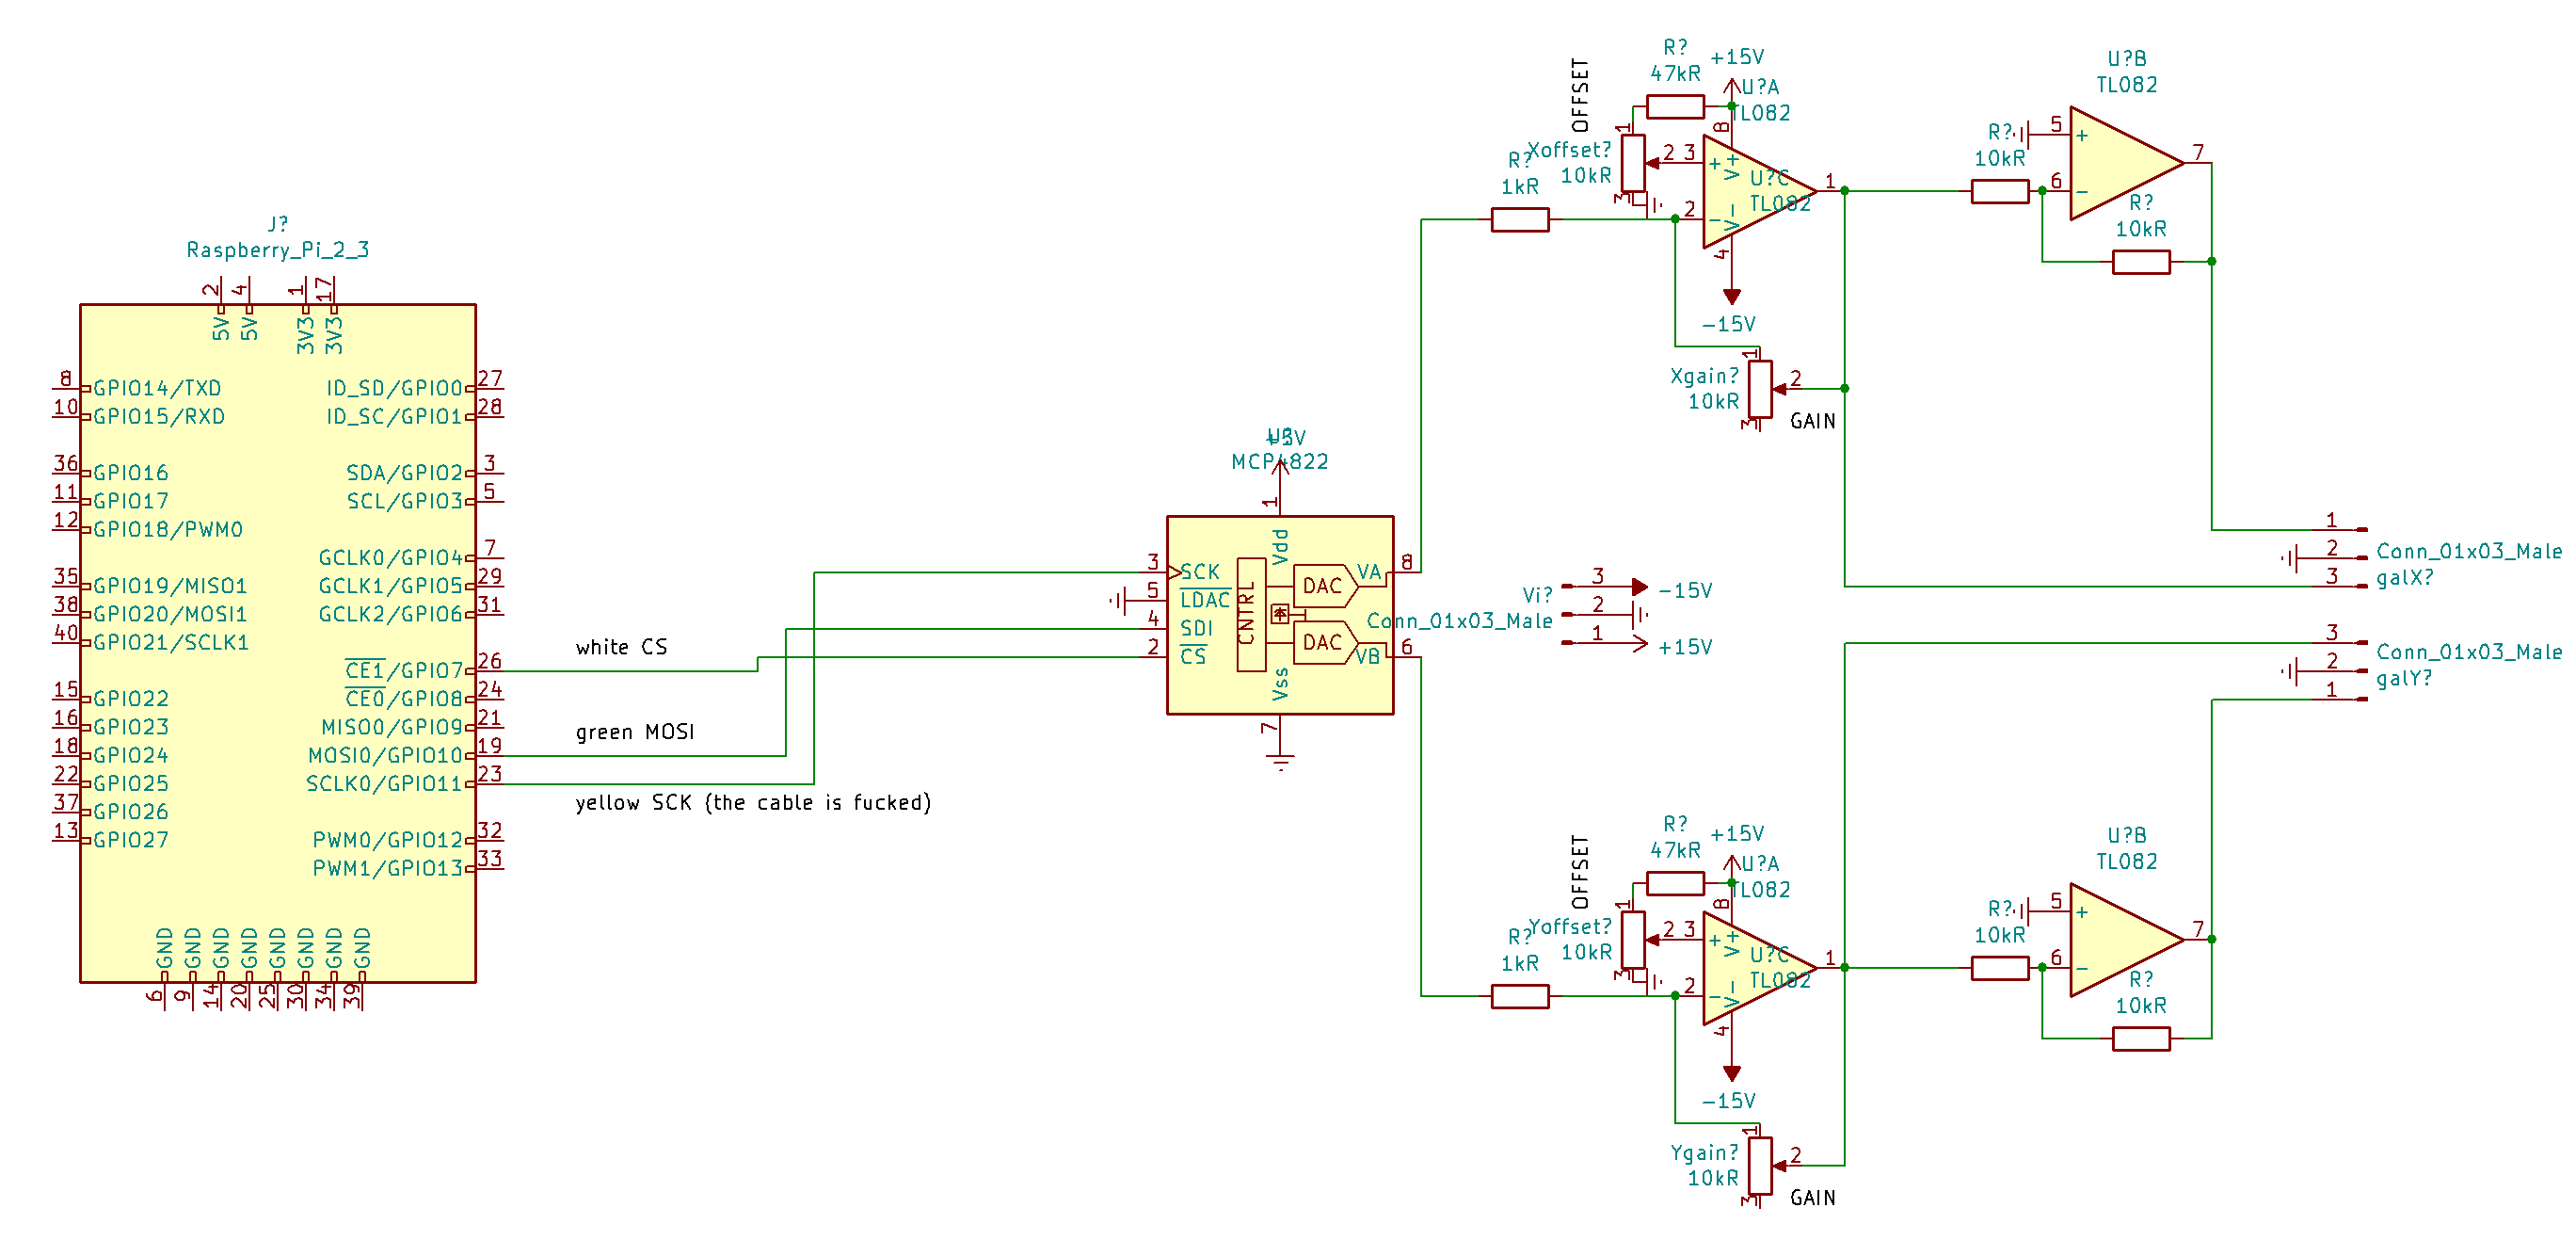
\includegraphics[width=1\textwidth]{img/dac_board.png} 
  \caption{\label{fig:dac_board}Zapojení DAC a zesilovačů k RPi a řídící desce galvanometrů}
\end{figure}

\subsubsection{dac}
K generování signálu v rozpětí 0--5~V jsem využil DAC MCP4822 od firmy \href{https://www.microchip.com}{Microchip Technology Inc.}\ \fxnote{TODO tečka? ("\textbackslash " == explicitni mezera)}
Tento čip podporuje komunikaci přes rozhraní SPI, pracuje s napájecím napětím 5~V a s 12bitovým rozlišením (je schopen vygenerovat 4~096 různých napětí) na dvou kanálech.

RPi komunikuje s čipem pomocí rozhraním SPI, toto rozhraní využívám pomocí knihovny ze serveru \url{https://github.com}\footnote{\url{https://github.com/abelectronicsuk/ABElectronics_CPP_Libraries/tree/master/ADCDACPi}; staženo 2.~1.~2024} \fxnote{TODO tečka?}
\fxnote{TODO more spec}
Tato knihovna poskytuje následující funkce, se kterými pracuji v mém kódu.
\begin{itemize}
\item
\lstinline[language=C]!bool mcp4822_initialize();!
\item
\lstinline[language=C]!bool mcp4822_set_voltage(mcp4822_channel_t channel, uint16_t value_mV);!
\item
\lstinline[language=C]!void mcp4822_deinitialize();!
\end{itemize}
\subsubsection{amps}
K rozšíření signálu z DAC jsem využil dva operační zesilovače TL082 od firmy \href{https://www.ti.com/}{Texas Instruments Incorporated}. Každý z nich je připojený na jeden kanál DAC čipu mcp4822.
\fxnote{TODO more spec}
Tyto čipy mi napěťové rozpětí zvýší z 0--5~V na $-15$~V až $+15$~V.

zesilovac - cteni baterek \url{https://is.muni.cz/el/sci/jaro2017/F5090/um/E17_P8.pdf}
